\documentclass[11pt]{article}
\usepackage[a4paper,margin=1in]{geometry}
\usepackage{graphicx}
\usepackage{booktabs}
\usepackage{longtable}
\usepackage{array}
\usepackage{hyperref}
\usepackage{float}
\usepackage{siunitx}
\usepackage{listings}
\usepackage{xcolor}

\hypersetup{
  colorlinks=true,
  linkcolor=blue,
  urlcolor=blue,
  citecolor=blue
}

\title{GPU PyFR PASS 1 -- NASA Hump Reconstruction on Purdue Gilbreth}
\author{OpenAI Codex workflow inside \texttt{nasa-hump2}}
\date{\today}

\begin{document}
\maketitle

\section{Objective}
GPU PyFR PASS 1 establishes a reproducible CUDA-backed PyFR workflow for the NASA two-dimensional wall-mounted hump case on Purdue RCAC Gilbreth. The goal of this pass is infrastructure and diagnostic honesty first: prove that PyFR can be installed in user space, submitted through Slurm on a GPU node, and advanced toward a hump reconstruction without borrowing any hidden benchmark solution data.

\section{Prior OpenFOAM Baseline Summary}
The repository already contains multiple OpenFOAM hump passes with official NASA Cp and Cf comparison. Two OpenFOAM checkpoints are the most relevant baselines for this GPU pass:
\begin{itemize}
  \item PASS 4 promoted SST continuation to 650 iterations: benchmark MAE \num{0.1659136747}.
  \item Later plain-SST continuation to 800 iterations: benchmark MAE \num{0.1547381028}.
\end{itemize}
These baselines already include the official machine-readable NASA Cp/Cf comparison pipeline and give the PyFR workflow a physically grounded reference point.

\section{PyFR Modeling Scope}
PyFR PASS 1 uses \texttt{ac-navier-stokes} on the CUDA backend. This is not the same governing-equation and closure package as the existing OpenFOAM steady RANS SST baseline. The comparison is therefore intentionally framed as a cross-method reconstruction attempt rather than a claim of SST equivalence. Any mismatch or failure is documented as a modeling or implementation limitation, not hidden.

\section{Gilbreth GPU Environment}
The exact environment is recorded in \texttt{documentation\_src/GPU\_PYFR\_PASS1\_ENVIRONMENT.md}. The verified stack used during PASS 1 was:
\begin{itemize}
  \item access path: \texttt{ssh gilbreth},
  \item scratch workspace: \texttt{/scratch/gilbreth/prabhu56/nasa-hump2-gpu-pyfr-pass1},
  \item compiler and MPI modules: \texttt{gcc/11.5.0}, \texttt{openmpi/4.1.6},
  \item CUDA module: \texttt{cuda/12.6.0},
  \item Python: \texttt{3.9.25},
  \item PyFR: \texttt{1.15.0},
  \item compute-node GPU seen in Slurm jobs: \texttt{NVIDIA A100-PCIE-40GB}.
\end{itemize}

\section{Workflow and Reusable Files}
PASS 1 added a full remote-execution pipeline around PyFR:
\begin{itemize}
  \item \texttt{scripts/setup\_gilbreth\_pyfr\_env.sh} creates the Gilbreth virtual environment and records environment details.
  \item \texttt{scripts/pyfr/generate\_pyfr\_meshes.py} builds the smoke mesh and the hump meshes with the same reconstructed lower wall and contoured upper wall used by the OpenFOAM passes.
  \item \texttt{scripts/pyfr/build\_gpu\_pyfr\_pass1\_case.py} generates PyFR configuration files and sampling manifests.
  \item \texttt{scripts/submit\_pyfr\_smoke\_gilbreth.sh}, \texttt{scripts/submit\_pyfr\_medium\_gilbreth.sh}, and \texttt{scripts/submit\_pyfr\_promoted\_gilbreth.sh} provide Slurm submission wrappers.
  \item \texttt{scripts/fetch\_gpu\_pyfr\_pass1\_results.sh} and \texttt{scripts/postprocess\_gpu\_pyfr\_pass1.py} pull lightweight results back into the repo and generate the PASS 1 figures and tables.
\end{itemize}

\section{Mesh and Case Reconstruction}
The PyFR hump geometry reuses the existing repository reconstruction choices:
\begin{itemize}
  \item chord length \SI{0.42}{m},
  \item lower hump wall represented by the repo's smooth cosine-squared hump,
  \item mild contoured upper wall retained to approximate blockage guidance from the allowed NASA sources,
  \item inlet located well upstream of the hump rather than directly at the first validation station.
\end{itemize}
The PASS 1 mesh path was deliberately incremental:
\begin{enumerate}
  \item a rectangular smoke mesh to validate the CUDA backend and Slurm path,
  \item a curved structured hump mesh,
  \item a structured triangular hump mesh,
  \item a piecewise-linear triangular hump mesh as a more robust fallback.
\end{enumerate}

\begin{figure}[H]
  \centering
  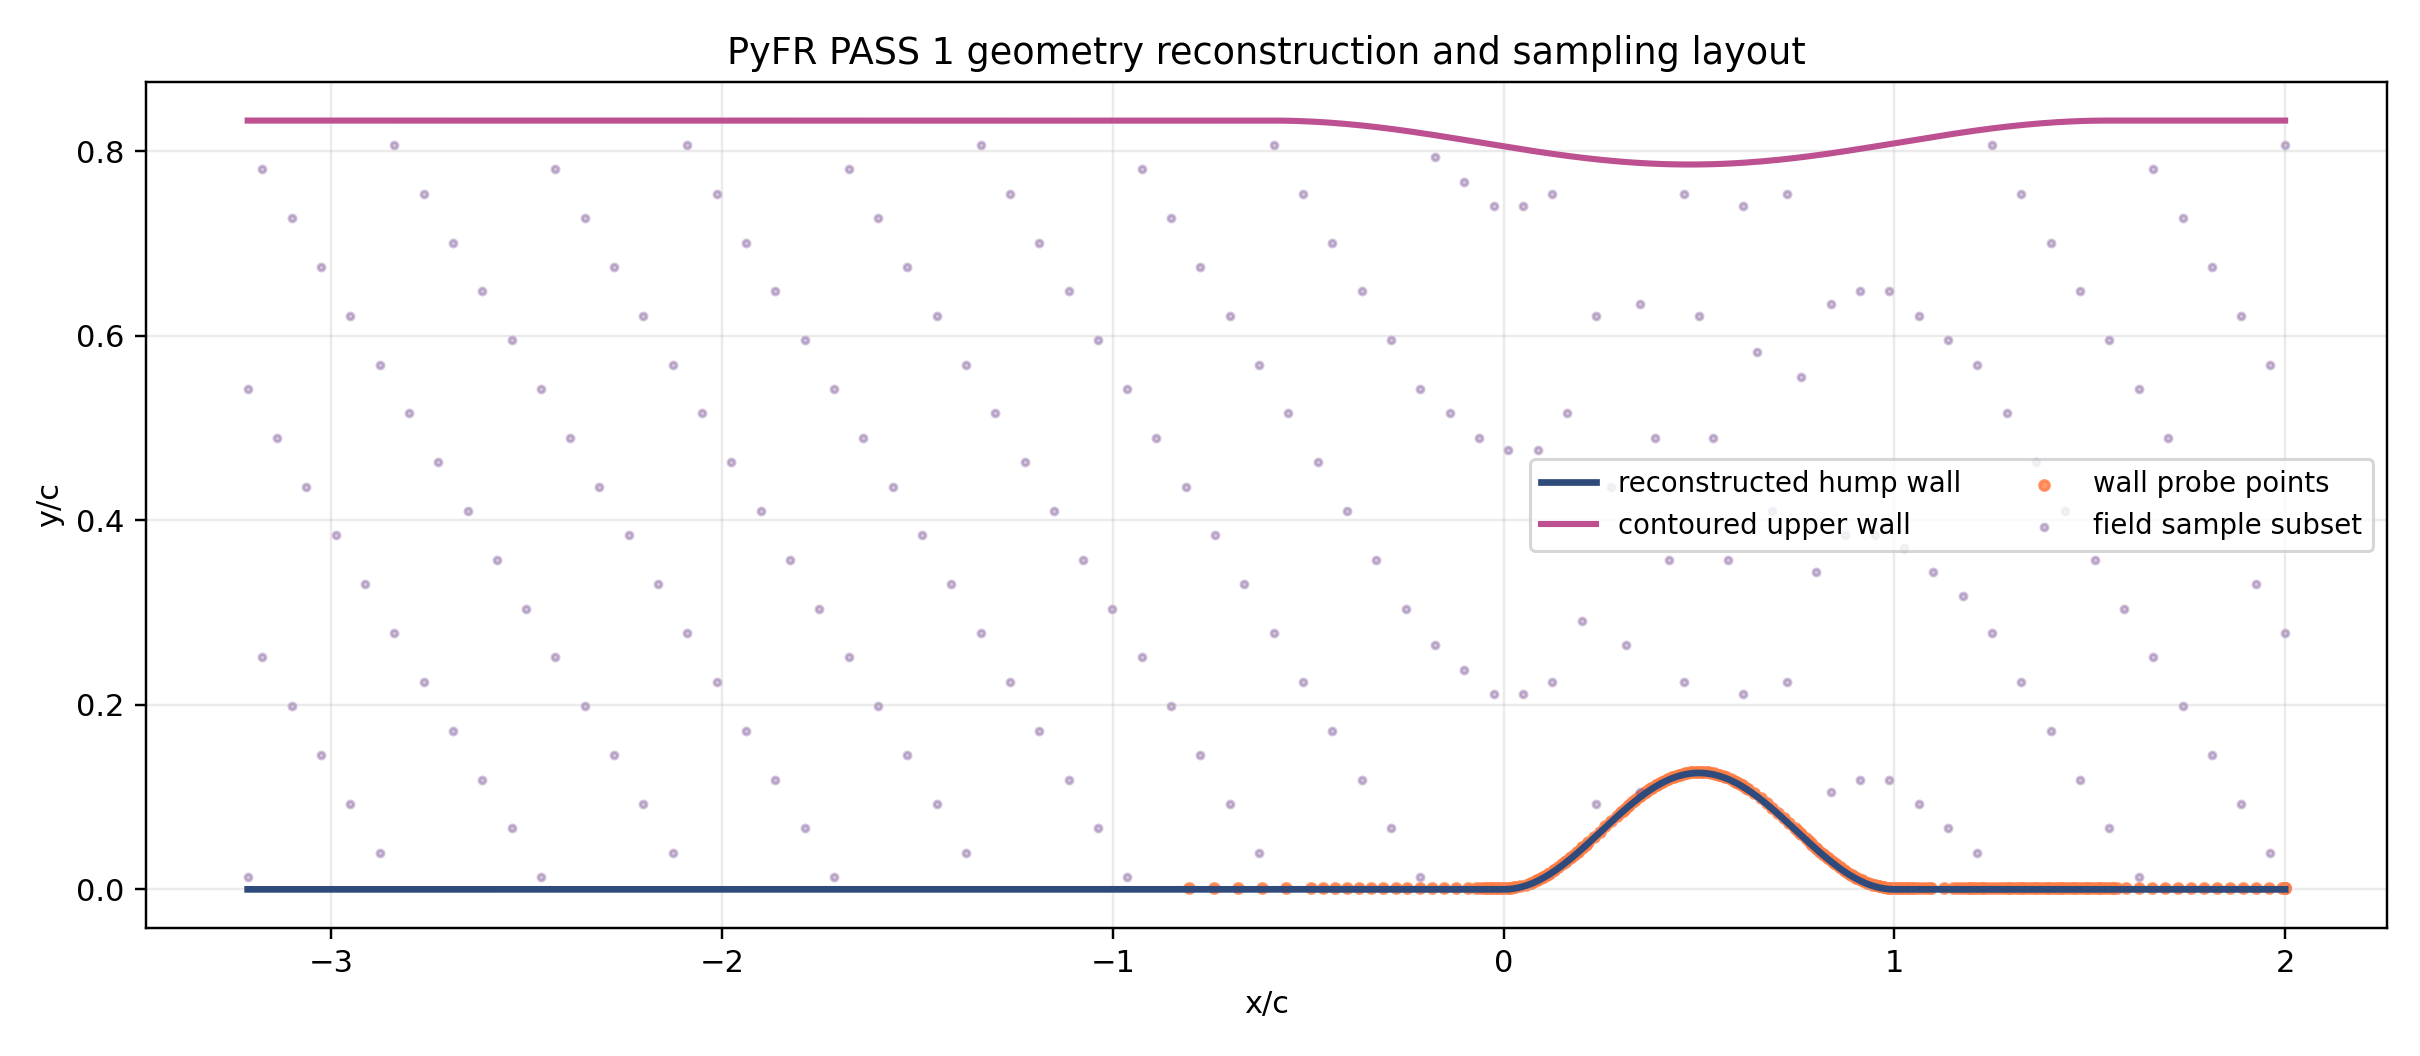
\includegraphics[width=\textwidth]{../figures_gpu_pyfr_pass1/pyfr_geometry_sampling.png}
  \caption{Geometry and sampling layout used to build the PyFR hump attempt. The lower wall and upper contour come from the repository's existing reconstruction logic, while the sample points are generated automatically from the local NASA comparison pipeline.}
\end{figure}

\section{PyFR Numerical Setup}
The generated PyFR configurations use:
\begin{itemize}
  \item \texttt{ac-navier-stokes},
  \item double precision,
  \item CUDA backend with \texttt{device-id = local-rank},
  \item \texttt{mpi-type = standard},
  \item dual-time integration,
  \item conservative first-pass polynomial orders and time-step settings,
  \item no-slip lower wall and slip upper wall,
  \item sampler plugins for wall, field, profile, and benchmark points on the hump runs.
\end{itemize}
Those settings were chosen to start from a numerically conservative baseline instead of attempting an overly aggressive production-quality run on the first GPU pass.

\section{Slurm Job Workflow}
All meaningful work was submitted through Slurm on the \texttt{a100-40gb} partition. The smoke test was required to succeed before escalating to the hump case. The promoted hump job was intentionally not submitted after the medium hump attempts exposed unresolved PyFR mesh/sampler issues.

\section{Run Results}

\subsection{Outcome Table}
\begin{center}
\scriptsize
\begin{tabular}{p{1.8cm} p{1.25cm} p{1.45cm} p{1.35cm} p{1.35cm} p{6.0cm}}
\toprule
Case & Status & Benchmark MAE & Cp MAE & Cf MAE & Notes\\
\midrule
OF PASS4 & completed & 0.165914 & 0.171180 & 0.000848 & Best PASS 4 continuation to 650 iterations.\\
OF SST800 & completed & 0.154738 & 0.164179 & 0.000768 & Strongest existing plain-SST baseline entering PyFR PASS 1.\\
OF PASS5 & completed & 0.135890 & 0.153755 & 0.000673 & Best local OpenFOAM benchmark after later continuation to 1200 iterations.\\
PyFR smoke & completed & -- & -- & -- & CUDA backend smoke test completed through Slurm; no NASA hump metrics expected.\\
PyFR curved & failed & -- & -- & -- & Failed during interface face-point sorting inside PyFR element/intersection setup.\\
PyFR tri & failed & -- & -- & -- & Structured triangle variant still failed in interface ordering before marching.\\
PyFR linear tri & failed & -- & -- & -- & Solver advanced beyond import/setup, but sampler plugin failed before evaluation and wall CSV export.\\
\bottomrule
\end{tabular}
\end{center}

\subsection{Attempt Status}
\begin{figure}[H]
  \centering
  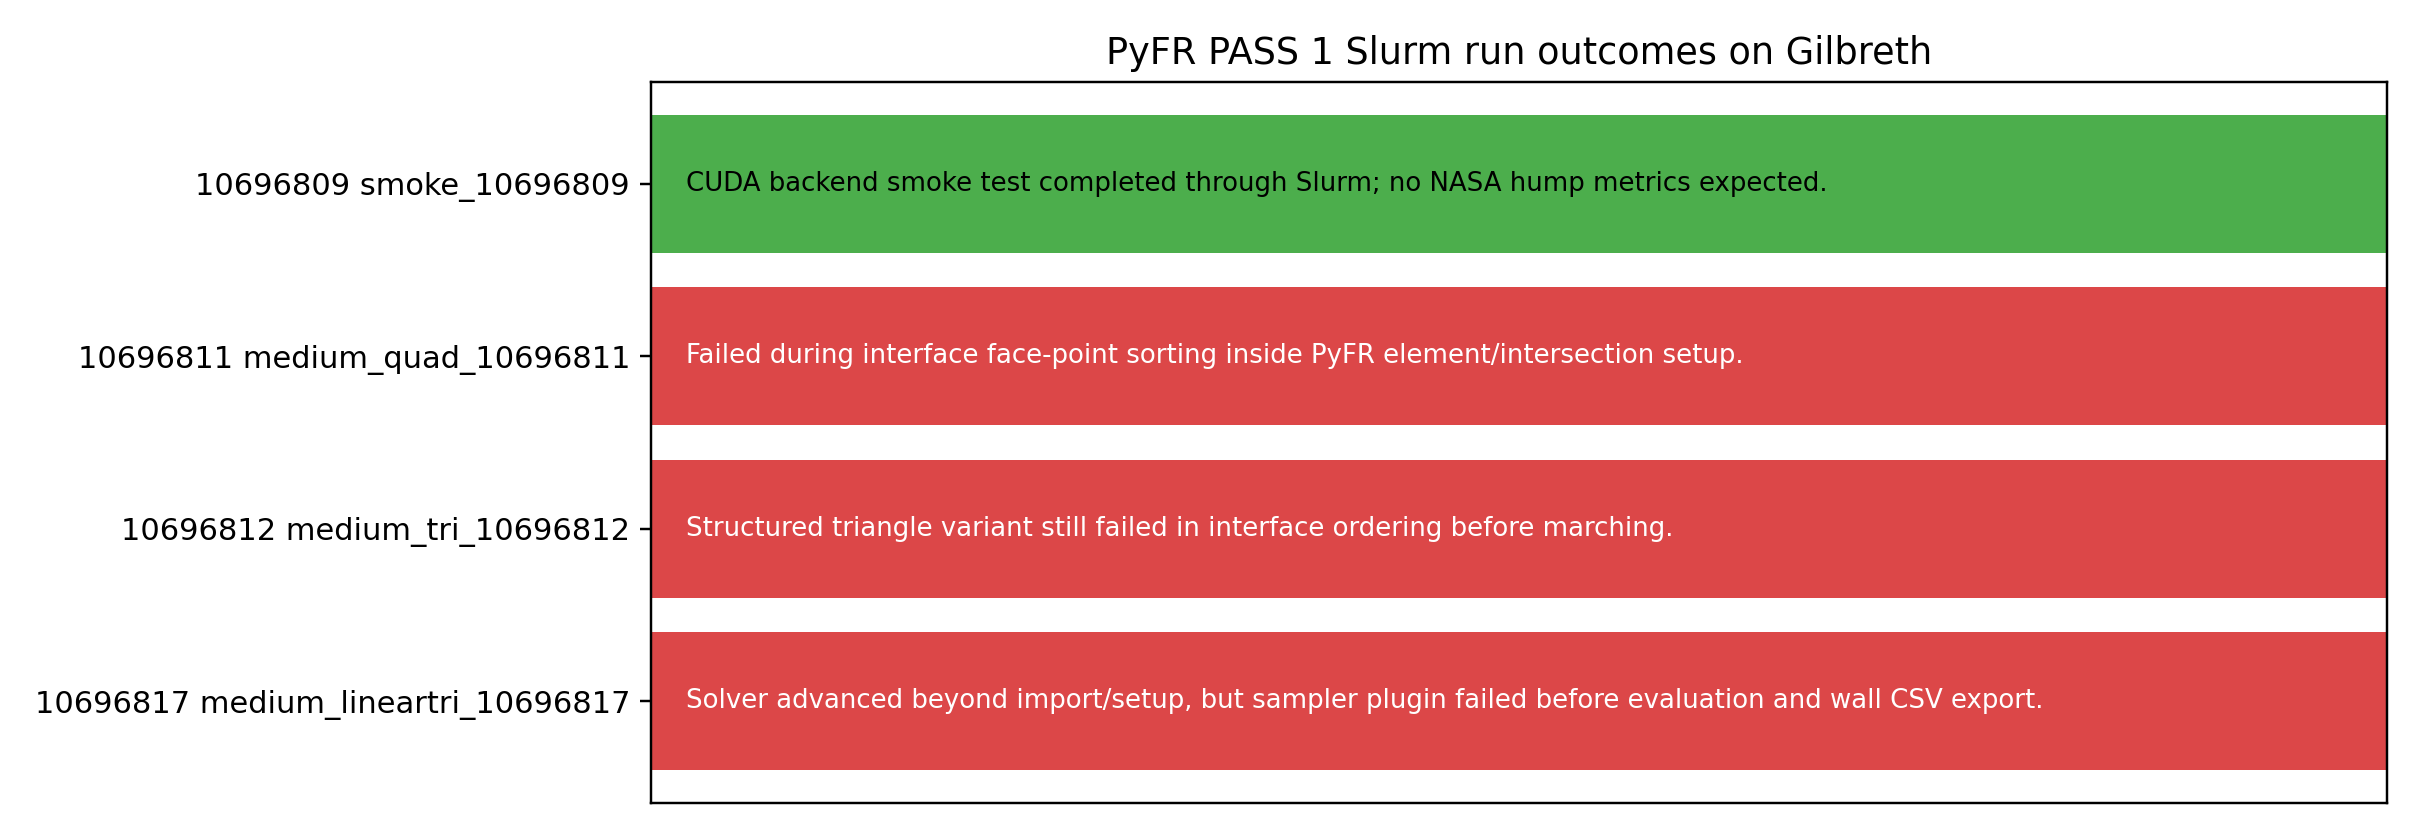
\includegraphics[width=\textwidth]{../figures_gpu_pyfr_pass1/pyfr_attempt_status.png}
  \caption{PASS 1 PyFR run outcomes. The smoke case completed on the GPU. The hump attempts progressively moved from mesh/interface failures to a later sampler-plugin failure after solver setup.}
\end{figure}

\subsection{Smoke-Test Diagnostics}
\begin{figure}[H]
  \centering
  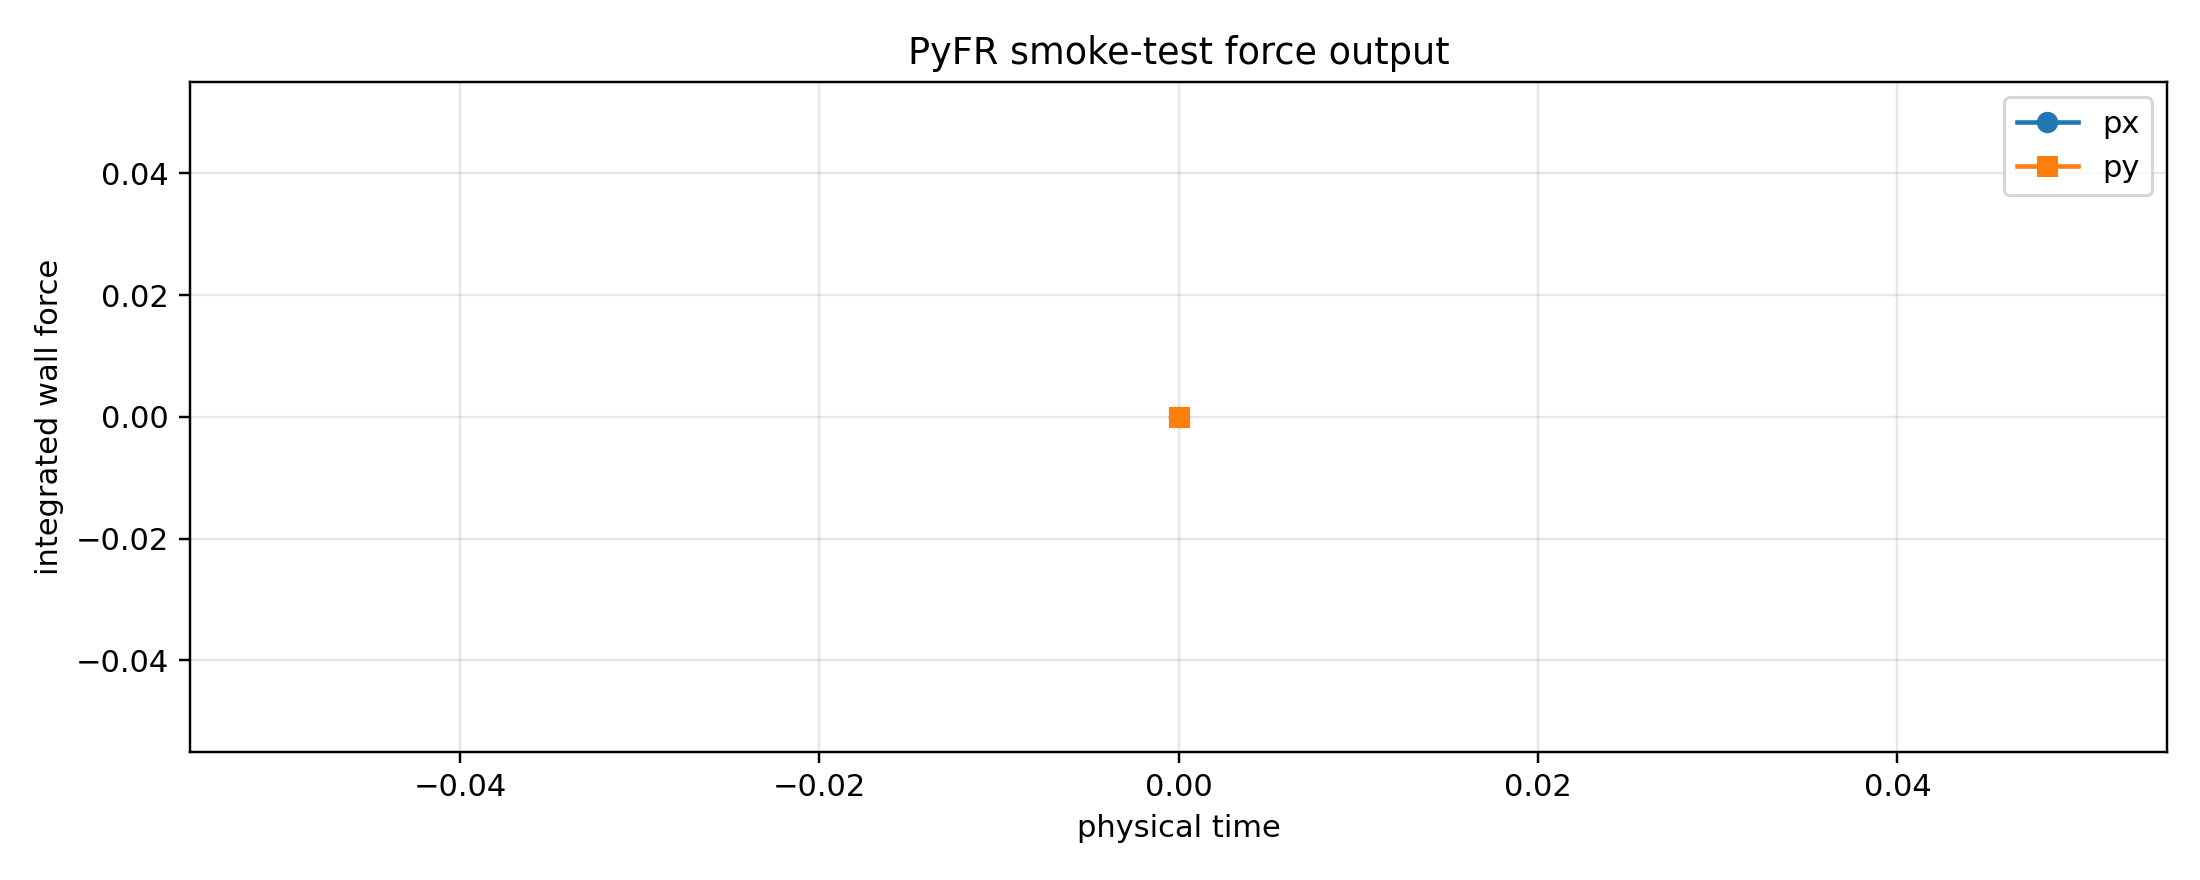
\includegraphics[width=\textwidth]{../figures_gpu_pyfr_pass1/smoke_force_history.png}
  \caption{Smoke-test force output. The result is useful primarily as a plugin-execution sanity check rather than a physically meaningful aerodynamic signal.}
\end{figure}

\section{Cp and Cf Comparison Against NASA Data}
PASS 1 preserved the official machine-readable NASA Cp and Cf import path, but the hump run did not reach a state where valid PyFR wall-distribution CSV files were written. Specifically, job \texttt{10696817} advanced beyond PyFR import and solver setup on the piecewise-linear triangular hump mesh, but then failed inside the sampler plugin when refining the requested sample-point set. Because of that, PASS 1 does \emph{not} claim a valid PyFR hump Cp or Cf curve.

\begin{figure}[H]
  \centering
  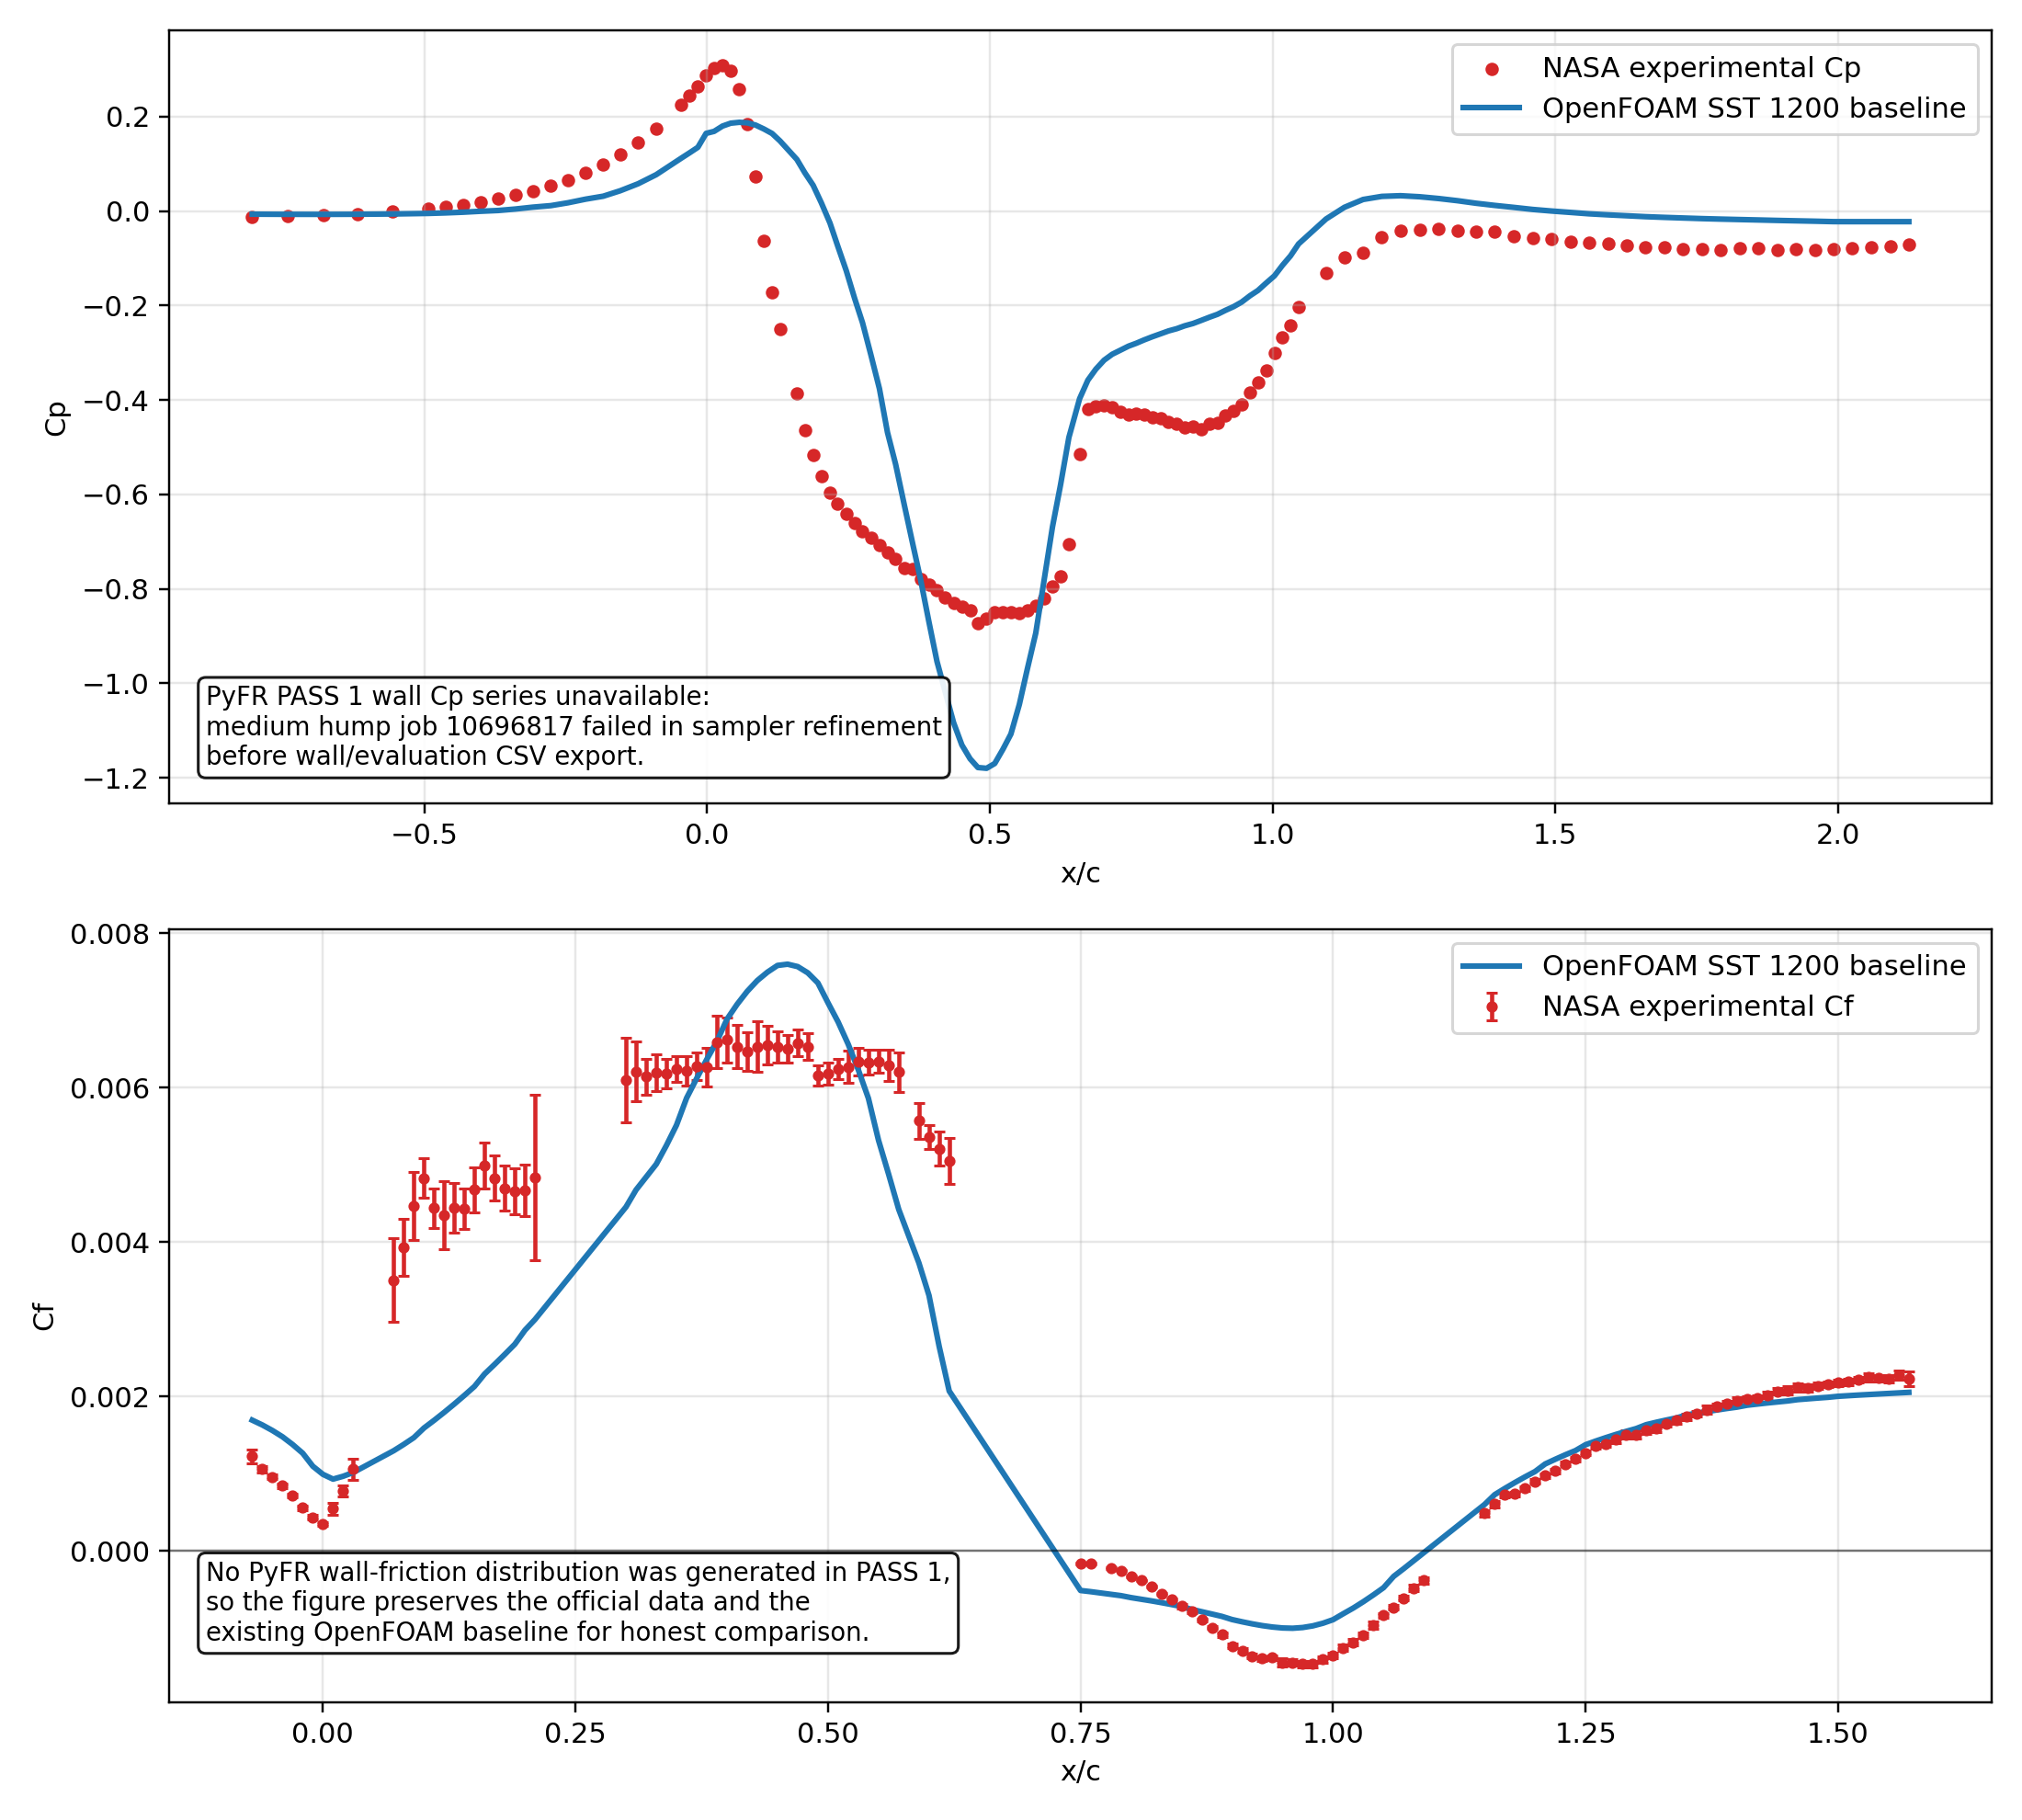
\includegraphics[width=\textwidth]{../figures_gpu_pyfr_pass1/cp_cf_vs_nasa_gpu_pyfr_pass1.png}
  \caption{Official NASA wall-coefficient data together with the best existing OpenFOAM baseline already present in the repository. PASS 1 did not produce a valid PyFR wall series, so the figure keeps the comparison honest instead of fabricating a PyFR overlay.}
\end{figure}

\section{Comparison Against the OpenFOAM Baseline}
The strongest OpenFOAM continuation already in the repository remains the reference standard for this problem. Relative to that baseline, GPU PyFR PASS 1 achieved the following:
\begin{itemize}
  \item successful user-space installation of PyFR on Gilbreth,
  \item successful Slurm GPU smoke test on an A100 node,
  \item successful reconstruction and import attempts for multiple hump mesh variants,
  \item one hump attempt that advanced into solver execution before failing in the sampler stage,
  \item no valid hump benchmark MAE, Cp MAE, or Cf MAE yet.
\end{itemize}
So PASS 1 is scientifically useful as a GPU-workflow baseline, but it is not yet competitive with the OpenFOAM hump benchmark.

\section{Failure Modes and Limitations}
The dominant PASS 1 limitations are:
\begin{itemize}
  \item PyFR PASS 1 does not reproduce OpenFOAM SST physics; it uses \texttt{ac-navier-stokes}.
  \item The curved and structured hump meshes failed in PyFR face-point sorting during interface setup.
  \item The linearized triangular hump mesh progressed further, but the sampler plugin failed before benchmark and wall-comparison CSV export.
  \item Without valid hump wall/evaluation output, PASS 1 cannot honestly quote a PyFR benchmark MAE against the NASA hump.
  \item The smoke-test plugin outputs contained only startup-level force information, which is enough for plumbing validation but not for aerodynamic interpretation.
\end{itemize}

\section{Reproducibility Commands}
\begin{lstlisting}[basicstyle=\ttfamily\small,breaklines=true]
cd /Users/ashmitprabhu/github/nasa-hump2
ssh gilbreth
cd /scratch/gilbreth/prabhu56/nasa-hump2-gpu-pyfr-pass1/repo_git
bash scripts/setup_gilbreth_pyfr_env.sh
bash scripts/submit_pyfr_smoke_gilbreth.sh
bash scripts/submit_pyfr_medium_gilbreth.sh

# Back on the local machine
cd /Users/ashmitprabhu/github/nasa-hump2
bash scripts/fetch_gpu_pyfr_pass1_results.sh
python3 scripts/postprocess_gpu_pyfr_pass1.py
tectonic -X compile documentation_src/gpu_pyfr_pass1/main.tex --outdir documentation
\end{lstlisting}

\section{Conclusion and Next-Step Recommendation}
GPU PyFR PASS 1 succeeded as an infrastructure pass and failed as a full hump benchmark pass, which is still a valuable result. The most promising next step is not arbitrary tuning; it is to remove or simplify the sampler dependency so that a hump solution can complete and be exported first, then reintroduce benchmark and wall probes in a more PyFR-compatible way. A second practical path would be to revisit the hump mesh construction with an even more PyFR-friendly element/topology strategy before spending more cluster time on higher-fidelity comparisons.

\bibliographystyle{plain}
\bibliography{references}

\end{document}
